\section{Colored Braided Operads}

In this section, we will define colored braided operads and will aim to find a op-fibration
that encodes all the necesaary data to define a colored braided operad.
First, let us recall the definition of $\Ex$ and build a related category $\Br$ 
that will serve as the base category for our op-fibration later on.

\begin{rem}
    For each $n \in \N$ we have an object $\langle n \rangle$. 
    A mophism $\langle n \rangle \to \langle m \rangle$ in $\Ex$ consists of a morphism 
    $\alpha \colon \langle n \rangle \to \langle m \rangle$ in $\Fin$ and a collection of configurations
    $$\{c_j \in \E_2(|\alpha^{-1}(j)|)\}_{1 \leq j \leq m}$$
    where each configuration is labeled by $\alpha^{-1}(j))$.
    So for example, 
    \begin{align*}
        \alpha \colon \langle 3 \rangle &\to \langle 2 \rangle \\
        1 &\mapsto 1 \\
        2 &\mapsto 2 \\
        3 &\mapsto 1 \\
    \end{align*}
    together with the configurations:
    \begin{center}
    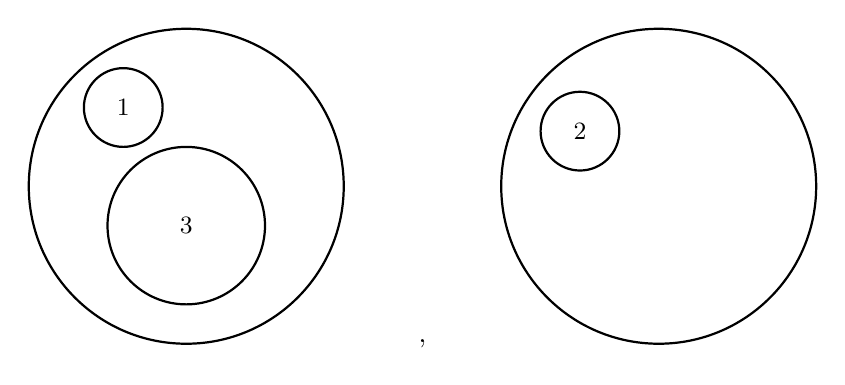
\begin{tikzpicture}
                        % First element (left)
                        \draw[thick] (-3,0) circle (2);
                        \draw[thick] (-3.8, 1) circle (0.5);
                        \draw[thick] (-3, -0.5) circle (1);
                        \node at (-3.8, 1) {\small $1$};
                        \node at (-3, -0.5) {\small $3$};
                        \node at (0,-2) {,};
                        % Second element (right)
                        \draw[thick] (3,0) circle (2);
                        \draw[thick] (2,0.7) circle (0.5);
                        \node at (2,0.7) {\small $2$};
        \end{tikzpicture}
    \end{center}
    We denote the trivial configuration with label $x$ by $\id^x \in \E_2(1)$.
    Further, recall the composition in $\Ex$. Let 
    \begin{center}
        $\alpha \colon \langle n \rangle \to \langle m \rangle$ 
        with configurations $\{c_j\}_{1 \leq j \leq m}$ 
    \end{center}
    and 
    \begin{center}
        $\alpha' \colon \langle m \rangle \to \langle l \rangle$ 
        with configurations $\{c'_k\}_{1 \leq k \leq l}$. 
    \end{center}
    Then, the configuration $c'_k$ is labeled 
    by $\alpha'^{-1}=\{j_1^{(k)}, \dots, j_p^{(k)}\}$. So, we obtain a configuration 
    \[
        \gamma(c'_k, c_{j_1}, \dots, c_{j_p})
    \]
    labeled by $(\alpha' \circ \alpha)^{-1}(k)$ for all $1 \leq k \leq l$ 
    giving us the well-defined composition $\alpha' \circ \alpha$
\end{rem}
\todo{define active morphism?}
Let $I$ be a finite set and . 
Then for any  $I$-labeled configuration $\widetilde{I}$ in $\E_2$,
in a sense we can also 
consider an active morphism in $\Ex$:
\[
    \alpha \colon I \to \langle 1 \rangle
\]
for $\widetilde{I}$.
\todo{define BR category. How to define objects?}

Next, we partially enrich $\Ex$ with the groupoid structure.
Note, that it might be possible to enhace $\Ex$ topologially which is
not of interest to us at this point.

\begin{defin}
    Let $\Br$ be the following partially $\Grp$-enriched category:
    \begin{enumerate}[(i)]
        \item The objects of $\Br$ are finite sets $\langle n \rangle$ for $n \in \N$ 
        % together with
        % a configuration $\widetilde{\langle n \rangle} \in \E_2(n)$.
        \item A morphism $\alpha \colon \langle n \rangle \to \langle m \rangle$ in $\Br$ consists of a morphism 
        $\alpha \colon \langle n \rangle \to \langle m \rangle$ in $\Fin$ and a collection of configurations
        $$\{\widetilde{\alpha}_j \in \E_2(|\alpha^{-1}(j)|)\}_{1 \leq j \leq m}$$
        where each configuration $\widetilde{\alpha}_j$ is labeled by $\alpha^{-1}(j)$.
        The composition is defined analogously to the composition map in $\Ex$.
        \item The set of active morphisms
        $$\acthom( \langle n \rangle, \langle 1 \rangle)$$
        is the groupoid of homotopy classes of path between configurations in $\E_2(n)$. 
        
         
        % and consists of a finite set $I$ and a collection of configurations $\widetilde{I}$ in $\E_2$ labeled by $I$.
    \end{enumerate}

\end{defin}


\begin{defin}
    A {\em colored braided operad} $\B$ consists of the following data:
    \begin{enumerate}[(i)]
        \item A collection $\{X,Y,Z; \dots\}$ of colors.
        \item Let $I$ be a finite set and $\widetilde{I}$ an $I$-labeled configuration in $\E_2$. 
        For a collection of colors $\{X_i\}_{i \in I}$ and a color $Y$ in $\B$, there is 
        a set \todo{set/groupoid?} 
        \[
            \Mul_{\B}^{\widetilde{I}}(\{X_i\}_{i \in I}, Y)
        \]
        called the set of morphisms from $\{X_i\}_{i \in I}$ to $Y$.
§
        \item Let $\alpha \colon I \to J$ be finite mape together with a collection of 
        configurations labeled by the preimages of $\alpha$, i.e. 
        $$\widetilde{\alpha} = (\widetilde{I_j})_{j \in J}$$
        where $I_j$ denotes the fiber over $j$ for all $j \in J$
        and a path of configurations $\eta$:
        \begin{center}
            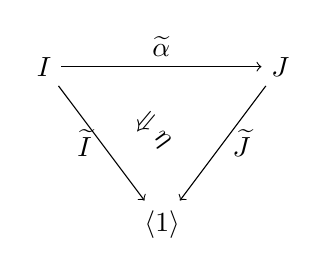
\begin{tikzpicture}
                % Define node positions
                \node (B) at (0, 2) {$I$};
                \node (C) at (3, 2) {$J$};
                \node (A) at (1.5, 0) {$\langle 1 \rangle$};
                
                % Draw arrows
                \draw[->] (B) -- (C) node[midway, above] {$\widetilde{\alpha}$};
                \draw[->] (B) -- (A) node[midway, left] {$\widetilde{I}$};
                \draw[->] (C) -- (A) node[midway, right] {$\widetilde{J}$};
                
                % Natural transformation arrow
                \node[rotate=-40] at (1.4, 1.2) {$\Downarrow \eta$};
                % \node at (1.7, 1.2) {$\eta$};
            \end{tikzpicture}
        \end{center}
        Further, let there be
        collections of colors $\{X_i\}_{i \in I}$ and $\{Y_j\}_{j \in J}$ and color $Z$. Then, 
        there is a composition map:
        \[
            \gamma \colon \prod_{j \in J} \Mul_{\B}^{\widetilde{I_j}}(\{X_i\}_{i \in I_j}, Y_j) \times \Mul_{\B}^{\widetilde{J}}(\{Y_j\}_{j\in J}, Z) \to \Mul_{\B}^{\widetilde{I}}(\{X_i\}_{i \in I}, Z)  
        \]
        \item There is a collection of morphisms $\{ \id_X \in \Mul_{\O}(\{X\}, X)\}_{X \in \O}$ being a left 
        and right unit in the composition, i.e. the following diagrams commute:
        \begin{center}
            \begin{tikzcd}
                {\Mul_{\B}^{\widetilde{I}}(\{X_i\}_{i \in I}, Y)} \arrow[r, "\cong"] \arrow[d, "\id"] & {\Mul_{\B}^{\widetilde{I}}(\{X_i\}_{i \in I}, Y) \times \{\id_Y\}} \arrow[d, hook]           \\
                {\Mul_{\B}^{\widetilde{I}}(\{X_i\}_{i \in I}, Y)}                                     & {\Mul_{\B}^{\widetilde{I}}(\{X_i\}_{i \in I}, Y) \times \Mul_{\B}^{\widetilde{Y}}((Y), Y)} \arrow[l, "\gamma"]
            \end{tikzcd}
        \end{center}
       
        \begin{center}
            \begin{tikzcd}
                {\Mul_{\B}^{\widetilde{I}}(X_I, Y)} \arrow[r, "\cong"] \arrow[d, "\id"] & {(\prod_{i \in I} \{\id_{X_i}\}) \times \Mul_{\B}^{\widetilde{I}}(X_I, Y)} \arrow[d, hook]           \\
                {\Mul_{\B}^{\widetilde{I}}(X_I, Y)}                                     & {(\prod_{i \in I} \Mul_{\B}^{\id^{i}}((X_i), X_i)) \times \Mul_{\B}^{\widetilde{I}}(X_I, Y)} \arrow[l, "\gamma"]
            \end{tikzcd}                                             
        \end{center}
        \item For every sequence of finite maps $I \overset{\alpha}{\to} J \overset{\beta}{\to} K$, 
        with paths

        \begin{center}
            \begin{tikzpicture}
                % Define node positions
                \node (B) at (0, 2) {$I$};
                \node (C) at (3, 2) {$J$};
                \node (A) at (3, -1) {$\langle 1 \rangle$};
                \node (D) at (6, 2) {$K$};

                % Draw arrows
                \draw[->] (B) -- (C) node[midway, above] {$\widetilde{\alpha}$};
                \draw[->] (C) -- (D) node[midway, above] {$\widetilde{\beta}$};
                \draw[->] (B) -- (A) node[midway, left] {$\widetilde{I}$};
                \draw[->] (C) -- (A) node[midway, right] {$\widetilde{J}$};
                \draw[->] (D) -- (A) node[midway, right] {$\widetilde{K}$};
                % Natural transformation arrow
                \node at (2.0, 1.1) {$\overset{\Leftarrow}{\eta}$};
                \node at (4.2, 1.1) {$\overset{\Leftarrow}{\epsilon}$};
            \end{tikzpicture}
        \end{center}
        % \begin{center}
        %     \begin{tikzcd}
        %         {\prod_{j \in J} \Mul_{\O}(X_I, Y_j) \times \prod_{k \in K} \Mul_{\O}(Y_J, W_k) \times \Mul_{\O}(W_K, Z)} \arrow[rd, "\id \times \gamma"] \arrow[dd, "(\gamma \circ s) \times \id"] & \\
        %                     & {\prod_{j \in J} \Mul_{\O}(X_{I_j}, Y_j) \times \Mul_{\O}(Y_J, Z)} \arrow[dd] \\
        %         {\prod_{k \in K} \Mul_{\O}(X_{I_k}, W_k) \times \Mul_{\O}(W_K, Z)} \arrow[rd] & \\
        %                     & {\Mul_{\O}(X_I, Z)}         
        %     \end{tikzcd}
        % \end{center}

        and collections of colors
        $X_I = \{X_i\}_{i \in I}$, $Y_J = \{Y_j\}_{j \in J}$, $W_K = \{W_k\}_{k \in K}$ and a color $Z \in \B$ 
        the following diagram commutes:
         \todo{make diagram prettier}
        \begin{center}
        \begin{adjustbox}{max width=\textwidth}
            \begin{tikzcd}
                {\prod_{j \in J} \Mul_{\B}^{\widetilde{I_j}}(X_{I_j}, Y_j) \times \prod_{k \in K} \Mul_{\B}^{\widetilde{J}}(Y_J, W_k) \times \Mul_{\B}^{\widetilde{K}}(W_K, Z)} \arrow[rd, "\id \times \gamma"] \arrow[dd, "(\gamma \circ s) \times \id"] & \\
                            & {\prod_{j \in J} \Mul_{\B}^{\widetilde{I_j}}(X_{I_j}, Y_j) \times \Mul_{\B}^{\widetilde{J}}(Y_J, Z)} \arrow[dd] \\
                {\prod_{k \in K} \Mul_{\B}^{\widetilde{I_k}}(X_{I_k}, W_k) \times \Mul_{\B}^{\widetilde{K}}(W_K, Z)} \arrow[rd] & \\
                            & {\Mul_{\B}(X_I, Z)}         
            \end{tikzcd}
            \end{adjustbox}
        \end{center}
    \end{enumerate}
\end{defin}